\documentclass{article}

\usepackage{fancyhdr} % Required for custom headers
\usepackage{lastpage} % Required to determine the last page for the footer
\usepackage{extramarks} % Required for headers and footers
\usepackage{graphicx} % Required to insert images
\usepackage{lipsum} % Used for inserting dummy 'Lorem ipsum' text into the template
\usepackage{ulem} % Required for Cross out text
\usepackage{amsmath} % Required for Math Stuff
\usepackage{amsfonts}
\usepackage{enumerate}
%\usepackage[]{algorithm2e}
\usepackage{hyperref}
%\usepackage{qtree}
\usepackage{hyperref}

\usepackage{caption}
\usepackage{subcaption}

% Margins
\topmargin=-0.45in
\evensidemargin=0in
\oddsidemargin=0in
\textwidth=6.5in
\textheight=9.0in
\headsep=0.25in
\setlength\parindent{0pt}

\linespread{1.1} % Line spacing

%----------------------------------------------------------------------------------------

\begin{document}

\title{Notes}
\author{Annie}
\maketitle
%%\vspace{-0.7in}

%----------------------------------------------------------------------------------------
%	Math Commands
%----------------------------------------------------------------------------------------

\providecommand{\abs}[1]{\left\vert#1\right\vert}
\providecommand{\norm}[1]{\left\Vert#1\right\Vert}

\section{Only Vertical Motion}

Lets say $a(t)$ describes the vertical motion of the pivot and $b(t)$ describes the motion of the following edge. In this case, $a(t)$ only moves in the $\hat{y}$ direction and $b(t)$ in the $\hat{x}$ direction. Our equations of motion can be given by 

\begin{equation}\label{eq:b}
b(t) = \sqrt{l^2 - a(t)^2}
\end{equation}

where $l$ is the length of the block. The velocity of $b$ is given by 

\begin{equation}\label{eq:db}
\dot{b}(t) = \frac{-a(t)\dot{a}(t)}{\sqrt{l^2 - a(t)^2}}
\end{equation}

If we assume, for now, that $b$ is a point contact with no friction, as long as $\dot{b}(t)$ is negative, $b$ will have momentum in the negative direction at $x=0$ and behave symmetrically after the flip. This simply requires $a(t)$ and $\dot{a}(t)$ to be the same sign. Since negative $a(t)$ would be into the table, this means they must both be postive. Our ideal motion is with the velocity of b being zero at both $x=l$ and $x=-l$ and largest at $x=0$. This occurs any monotonically increasing $a(t)$

\section{Assumptions}

\begin{itemize}

  \item Friction with the table
  \item Friction at the fingers
  \item Shape of the block
  \item Acceleration limits of the arm
  \item Mass distribution of the block

\end{itemize}

\section{Breaking the Assumptions}

\begin{itemize}

  \item Friction with the table 

    If there is too much friction between the block and the table 

  \item Friction at the fingers

    If there is too much friction from the fingertips, the object won't rotate.

  \item Shape of the block 
    \begin{itemize}
    \item Certain shapes require more than just length of the support face

    \begin{figure}[h!]
      \centering
      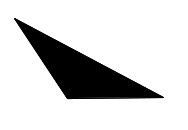
\includegraphics[width=0.25\textwidth]{triangle_failure.png}
      \caption{Need whole shape. Not just length of support face}
    \end{figure}

    \item Some faces can't be support faces

      \begin{figure}[h!]
        \centering
        \begin{subfigure}[b]{0.2\textwidth}
          
\includegraphics[width=\textwidth]{star.png}
        \end{subfigure}
        \begin{subfigure}[b]{0.2\textwidth}
          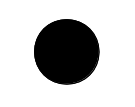
\includegraphics[width=\textwidth]{circle.png}
        \end{subfigure}
        \begin{subfigure}[b]{0.2\textwidth}
          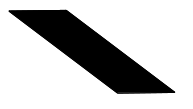
\includegraphics[width=\textwidth]{parallelogram.png}
        \end{subfigure}
        \caption{Tricky shapes}
      \end{figure}

      \end{itemize}
      
  \item Acceleration limits of the arm
  \item Mass distribution of the block

     \begin{figure}[h!]
        \centering
        \begin{subfigure}[b]{0.3\textwidth}
          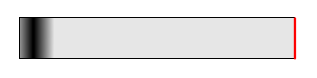
\includegraphics[width=\textwidth]{rectangle_weighted.png}
        \end{subfigure}
        \begin{subfigure}[b]{0.3\textwidth}
          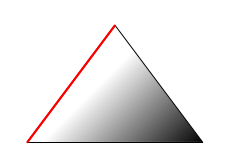
\includegraphics[width=\textwidth]{weighted_triangle.png}
        \end{subfigure}
        \caption{Non-uniform mass distribution }
      \end{figure}

\end{itemize}

\end{document}
